Es un punto mínimo que alcanza una onda al desplazarse. El punto más bajo, donde la amplitud es mínima.

Es el punto más alejado de la posición de equilibrio en la dirección negativa del desplazamiento.

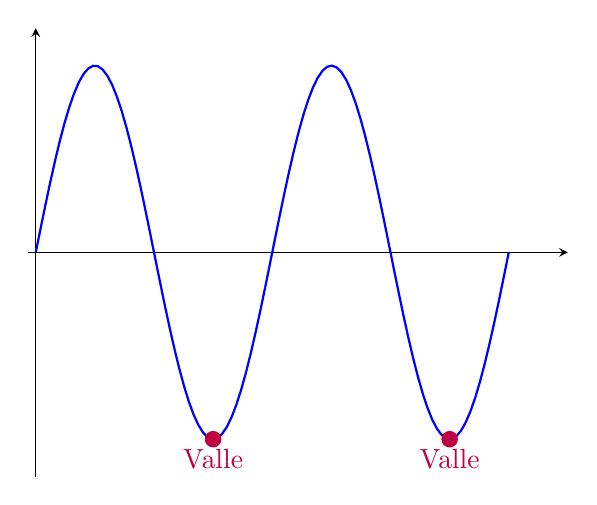
\begin{tikzpicture}
  \begin{axis}[
    xmin=-0.2,xmax=4.5*pi,
    ymin=-1.2,ymax=1.2,
    axis lines=middle,
    xtick={0},
    ytick={0}
    ]

    % Funcion senoidal
    \addplot[color=blue,samples=100,domain=0:4*pi,thick]{sin(deg(x))};

    % Valle 1
    \fill[purple] (axis cs:3*pi/2,-1) circle[radius=3pt];
    \node[purple,below] at (axis cs:3*pi/2,-1) {Valle};

    % Valle 2
    \fill[purple] (axis cs:7*pi/2,-1) circle[radius=3pt];
    \node[purple,below] at (axis cs:7*pi/2,-1) {Valle};
  \end{axis}
\end{tikzpicture}
